%%%%%%%%%%%%%%%%%%%%%%%%%%%%%%%%%%%%%%%%%%%%%%%%%%%%%%%%%%%%%%%%%%% 
%                                                                 %
%                            CHAPTER THREE                          %
%                                                                 %
%%%%%%%%%%%%%%%%%%%%%%%%%%%%%%%%%%%%%%%%%%%%%%%%%%%%%%%%%%%%%%%%%%% 
  
\chapter{Methods} \label{sec:methods}

In this chapter, we describe in detail the humpback fluke trailing edge algorithm pipeline.
We also briefly discuss some alternative approaches that we found to have limited successs.

\section{Trailing Edge Extraction}

Extracting good, high quality trailing edges images is one of the primary challenges when matching Humpback whales by their trailing edge.
In this section, we describe the steps that go into automating the extraction of high quality trailing edges.

One major assumption we make when extracting these trailing edges is that the humpback whale fluke is aligned such that its major axis is horizontal.
Additionally, we generally assume that all parts of the fluke are present.
The nature of the problem (and the dataset that we had at hand) makes these assumptions reasonable.
It would also be possible to add a detection step beforehand to ensure this assumption, however we do not explore this in this work.

\subsection{Fluke keypoint prediction}


\begin{figure*}[t]%
\centering
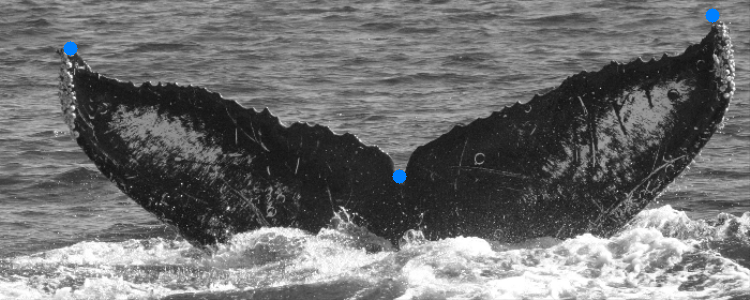
\includegraphics[width=1.0\textwidth]{../images/aid88_kpoverlay.png}
\caption{\textbf{Example Keypoint Prediction}. Example image showing the left tip, bottom of the notch, and right tip located by the keypoint extractor convolutional network.}
\label{fig:example_kp}
\end{figure*}

When extracting trailing edges, one of the first steps we take is to identify the starting and ending points of the trailing edge, as well as the bottom of the central notch.
To do this, we train a convolutional network to predict these three points.

The convolutional network does not need full-sized images, so the first step of the keypoint extraction pipeline is to resize the image to $256 \times 256$ pixels.
This size choice is somewhat arbitrary, but we find that it provides strong performance without using an unnecessary amount of memory.
The network predicts the points as values between $0$ and $1$, essentially giving coordinates into the image as percentages of its height and width. 
These predictions are then then rescaled back up to the original image size by multiplying with the original image height and width.
An example prediction is shown in Figure \ref{fig:example_kp}.

\subsubsection{Network Design}

The overall design of the network follows the pattern of alternating small ($3 \times 3$) convolutional filters with $2 \times 2$ max pooling layers, at each step doubling the number of channels (starting with $8$ channels).
This is somewhat similar to VGG-16 \cite{simonyan2014very}, although with half the trainable layers.
After a $32\times$ downsample has been achieved, we attach a decision layer which consists of a dense layer followed by three separate dense layers with separate predictions layers after (one for each point being predicted).
While this is not a common approach in keypoint prediction, we found that it gave better performance than having the points predicted as a single vector.
We theorize that this may be because shared units between each of the three predictions leads to stronger correlations between them, reducing overall prediction flexibility.

\subsubsection{Training Details}

Generating the training data for this is straightforward given a set of annotations with the associated points to learn.
The dataset that we created for this purpose contains approximately $2100$ training images, $700$ validation images, and $900$ test images.

First, each image is resized to a fixed width while maintaining the aspect ratio.
This is done to somewhat normalize the relative scale of objects in each image on the assumption that they are constrained to contain the fluke.
Each image is rescaled to the network size, and then the corresponding targets are rescaled to the range $[0-1]$.
The size of the original image is recorded as well.
The loss function that we use for each point is the Euclidean distance between the target and predicted point.
We also include a scalar scaling factor $\alpha$, which scales each point by a proportion of the original image size $\vec{s}$.
Thus, we have the scaled Euclidean loss $SE$

\begin{equation} \label{eqn:se_loss}
SE(\vec{t}, \vec{p}, \vec{s}, \alpha) = \lVert (\alpha * \vec{s}) \odot (\vec{t} - \vec{p}) \rVert
\end{equation} 
Where $\vec{t}$ and $\vec{p}$ are the target and predicted coordinates respectively \footnote{$\odot$ denotes elementwise multiplication}.
We then average this loss function over each point that the network predicts.

The networks are trained for 1000 epochs with $\alpha$ set to \num{2e-2} using the Adam \cite{kingma2014adam} optimizer (with recommended settings) and $l2$ regularization on the trainable parameters with a decay of \num{1e-4}.
All of these hyper parameters were tuned using the validation set, although the possible parameter space was not fully explored due to time constraints.

\subsubsection{Evaluation} 

% Problem is recreating all these experiments / networks for evaluation :/
% Might take a while...

On average, the best network achieved a 10 pixel distance error on the validation and testing sets (in the original image scale).
While this may seem like a lot, the trailing edge extraction (and subsequent matching accuracy) was not severely affected when only using the start and end point predictions.

We find that, for the vast majority of images, the network achieves a low pixel distance error, while there are a few that have a much higher error (see Figure \ref{fig:kp128_dist_hist}).
Qualitative inspection of these images shows that they are either of flukes which are not the singular or major object in the image, or flukes that are significantly rotated out-of-plane relative to the camera.
An example of this is shown in Figure \ref{fig:example_kp_failure}.

\begin{figure*}[t]%
\centering
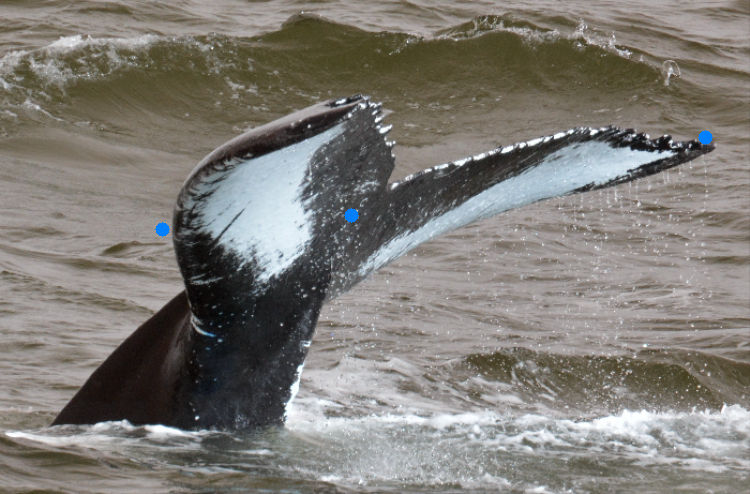
\includegraphics[width=1.0\textwidth]{../images/aid1323_kpoverlay.png}
\caption{\textbf{Example Keypoint Failure}. Example image showing a keypoint extraction failure case from its testing set. Note the difference in pose of the fluke from the success case shown in Figure \ref{fig:example_kp}. This is an example of a fluke image that violates our assumptions.}
\label{fig:example_kp_failure}
\end{figure*}



We attempted to use a spatial transformer network \cite{jaderberg2015spatial} to try and handle these cases, but we were unable to get it to perform as well as the standard convolutional network, nor produce sensible transformations.
Since these failure cases represent a small amount of the dataset, it is both difficult to train a network to handle them, and simultaneously not a large issue.
Additionally, we find that keypoint extraction failures are only a small percentage of the matching failure cases that we encounter.

\begin{figure*}[t]%
\centering
\includegraphics[width=1.0\textwidth]{../images/results/kp128_test_dist_hist.png}
\caption{\textbf{Histogram of Keypoint Distances}. This is a histogram of the average distance from predicted keypoints to annotated keypoints on the testing set for the keypoint extraction network. The vast majority of keypoints are predicted within 10 pixels of the true keypoints.}
\label{fig:kp128_dist_hist}
\end{figure*}



\subsection{Basic Trailing Edge Extraction Algorithm}


\begin{figure*}[t]%
\centering
\subfloat[][$I_y$]{
	\includegraphics[width=1.0\textwidth]{../images/aid88_vertgrad.png}
}
\newline
\subfloat[][Extracted Trailing Edge]{
	\includegraphics[width=1.0\textwidth]{../images/aid88_te_kp_overlay_noscorer.png}
}
\caption{\textbf{Example Trailing Edge Extraction}. Example of the baseline trailing edge extraction with $n = 2$. Note that the gradient image has a significant black area where the trailing edge is, making this an easy case.}
\label{fig:example_te_extract_noscorer}
\end{figure*}

The base algorithm for extracting the trailing edge uses the vertical gradient information of the image (denoted as $I_y$).
We extract $I_y$ using a vertically oriented $5 \times 5$ Sobel kernel \cite{Sobel1968}.  

Then we normalize $I_y$ with min-max scaling, giving $N_y$ as

\begin{equation} \label{eqn:norm01}
N_{y} = \frac{I_y - \min(I_y)}{\max(I_y) - \min(I_y)}
\end{equation}

Given $N_y$, we extract a trailing edge starting at the left tip of the fluke (a point denoted $s$) and ending at the right tip (a point denoted $e$).
To do this, we scan each pixel $(i,j)$ in $N_y$ starting from the column $s_x + 1$ and ending at the column $e_x$, updating a cost matrix $C$ cost with the following recursive update rule:

\begin{equation} \label{eqn:te_update}
C(x,y) = 
\begin{cases}
	0 & x < 0 \\
	\infty & y < 0 \text{ or } y > h \\
	\min_{y - \frac{n}{2} \leq y_c \leq y + \frac{n}{2}}C(x-1, y_c) + N_y(x,y) & \text{else} \\
\end{cases}
\end{equation}

Where $n$ is a neighborhood constraint and $h$ is the height of $N_y$.  
We default $n$ to $3$, meaning that each pixel considers its immediate ``neighbors'' from the previous column.

As $C$ is filled out, we also keep a backtrace matrix $B$, which keeps track of the index of the minimal candidate neighbor chosen in equation \eqref{eqn:te_update}.

\begin{equation} \label{eqn:backtrace_update}
	B(x,y) = \text{argmin}_{-n \leq n_c \leq n} C(x-1, y+n_c)
\end{equation}

Once the end column is reached, we scan the columns in reverse order from $e$ to construct the path by adding the chosen neighbor from $B$ at each step.
More formally, we start the trailing edge sequence $TE^0$ at $(e_x, e_y)$, and add elements to $TE$ as follows

\begin{equation} \label{eqn:te_build}
	TE^i = (TE^{i-1}_x - 1, (TE^{i-1})_y + B(TE^{i-1}_x,TE^{i-1}_y))
\end{equation}

In order to enforce that the path begins at $s$, we apply the following process before running the above.

\begin{align} \label{eqn:te_setup}
N_y(s_x,\cdot) = \infty \\
N_y(s_x,s_y) = 0
\end{align}

This forces the path to start at $s$, as otherwise it would take on infinite cost.
We optionally do the same for the point denoting the bottom of the notch, although we find that this can affect matching accuracy negatively if it is too far from the trailing edge.

An example of the base algorithm's output is given in Figure \ref{fig:example_te_extract_noscorer}.
While this algorithm has no understanding of humpback whale flukes, it generally finds high quality trailing edges in images that are constrained around the fluke with oceanic backgrounds (which is a large majority of the dataset at hand).
In the next section, we outline our approach for trying to make this more robust.


\subsection{Trailing Edge Scoring}

As mentioned in the beginning of this section, using only the gradient information for extracting the trailing edge works in many cases, but is not a robust method.

If we had a score of each pixel's ``trailing edginess'' in an image, the trailing edge extractor could make use of this information to make better choices in trailing edge extraction.
An example of this at work is shown in Figure \ref{fig:dis_te_use}.
To do this, we need a prediction of whether or not each pixel belongs to the trailing edge of a fluke --- a task that is best suited to a fully convolutional network.

In the fully convolutional networks that we use, we learn ``same'' convolutional kernels at each layer so as to maintain spatial shape from one layer to the next, except at explicit downsampling layers.
In order to construct a ``same'' kernel, we use square kernels of size $k \times k$ such that $k$ is odd, and apply them with a stride of $1$ in each direction.
Then, in order to ensure that the size of the output is the same as the size of the input, we add a zero-padding of size $\lfloor \frac{k}{2} \rfloor$ pixels to each side (filling in the corners).
In the networks used for trailing edge scoring, all convolutions (aside from the downsampling, i.e.\ max pooling layers) are ``same'' convolutions,
The four major variants on trailing edge scoring networks that we evaluated are detailed below.
All of these networks function on the same paradigm of taking an arbitrarily sized image and producing an image of the same size but with a class score for each pixel.

The dataset was sourced from trailing edges extracted using the basic method detailed above, however with manual adjustments to fix many of the more common issues we encountered with this algorithm.
These manual adjustments often included manually adding ``control points'', which forced the trailing edge through a specific point and often fixed major failures.
Additionally small adjustments were made that would not be found by the gradient finding algorithm.
Due to the extensive manual effort required to annotate and correct these images, only about $500$ images were annotated, many of which required little to no manual adjustments.
With these manually corrected trailing edges, we generated the training set for trailing edge scoring by extracting a $128 \times 128$ patch at $128$ pixel intervals along the trailing edge (giving a positive patch), and a corresponding patch (with no trailing edge pixels) randomly sampled from the left over space above and below the trailing edge (giving a negative patch).
As the images that this dataset were extracted from were generally $960$ pixels in width (with the trailing edges being only slightly smaller), on average about 15 patches were extracted from each image. 
These patches are then randomly split into training, testing, and validation sets each with $3700$, $1200$, and $1600$ patches respectively.


\begin{figure*}[t]%
\centering
\subfloat[][]{
	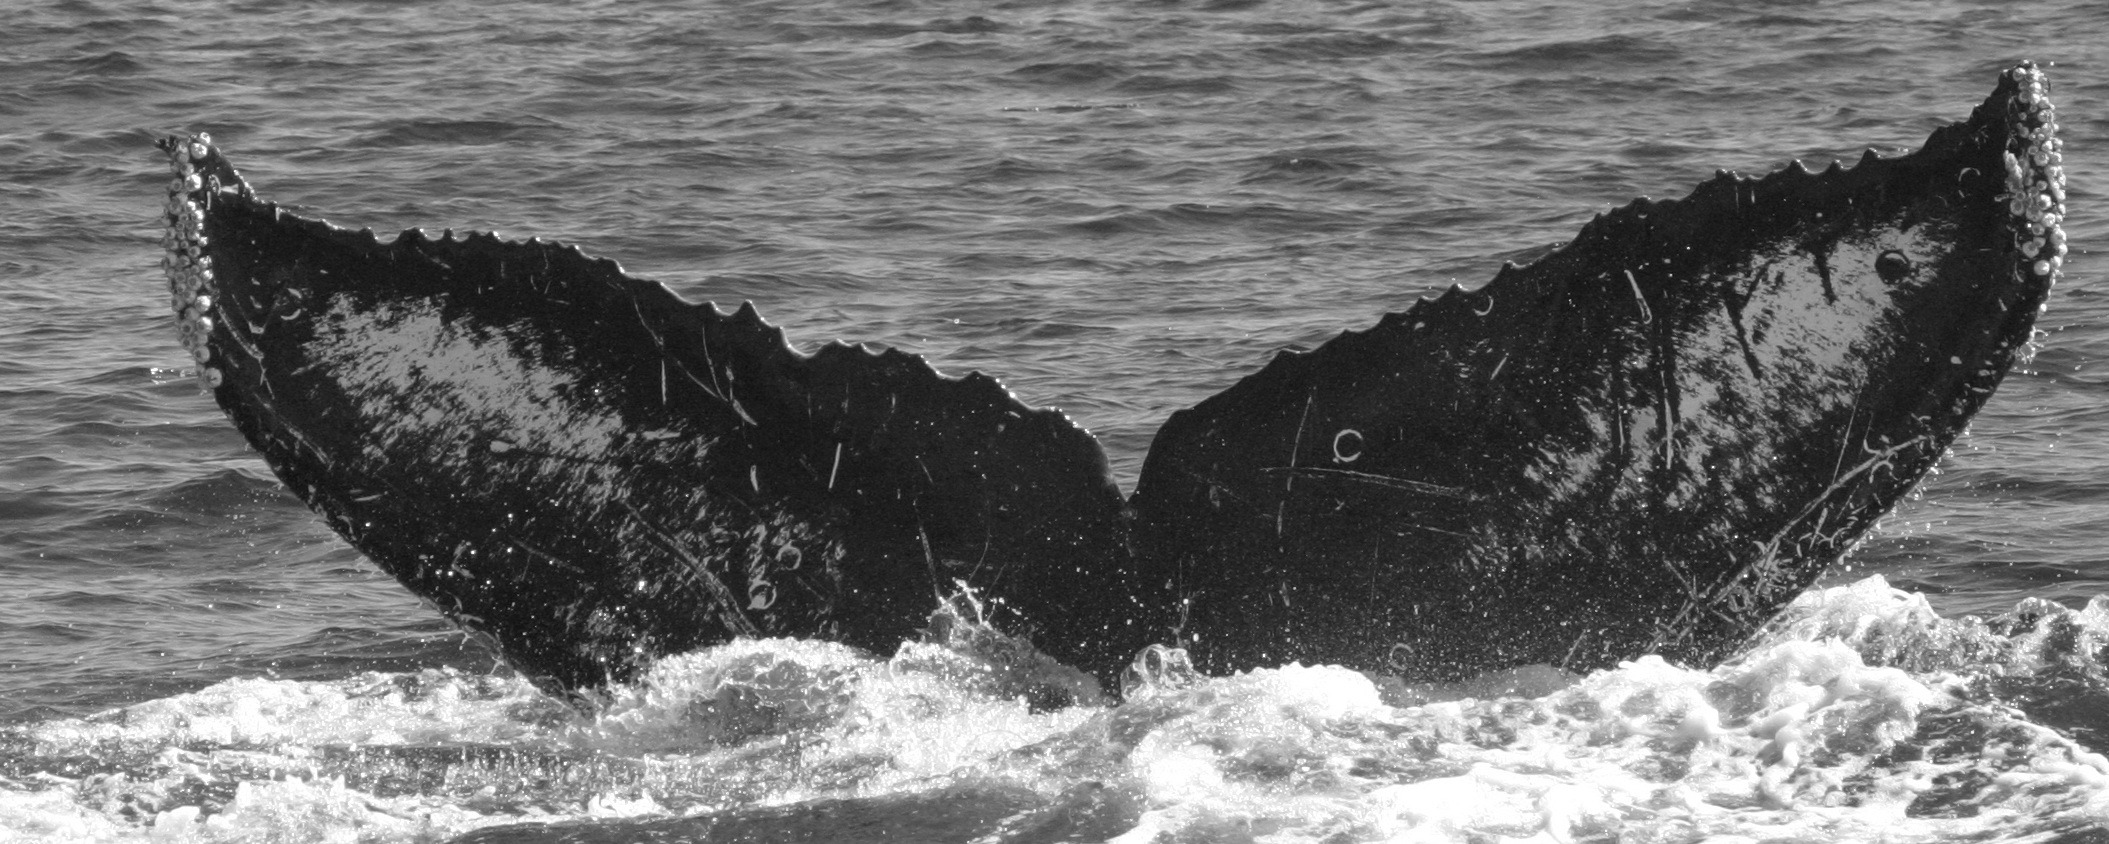
\includegraphics[width=1.0\textwidth]{../images/fluke_aid88_goodmatching.jpg}
}
\newline
\subfloat[][Trailing Edge Scores]{
	\includegraphics[width=1.0\textwidth]{../images/aid88_tescorer_annot_res.png}
}
\caption{\textbf{Example Trailing Edge Score}. Bottom image is the Residual scorer's classification of the top image. Trailing edge is class is colored black.}
\label{fig:example_te_score_annotres}
\end{figure*}



\subsubsection{Trailing Edge Scoring Architectures} 
\label{sec:te_arch}

Several network architectures were tried, although here we only report the major variants.
One major consideration that has to be made when selecting a fully convolutional network architecture is its receptive field\footnote{The receptive field of a convolutional network is, at a high level, the region of input that affects the output at a given layer}.
If the receptive field is too small, it may not have enough information to accurately determine if a given pixel is part of the trailing edge.
However, in order to increase the receptive field without massively increasing the depth of a network, we must downsample, which makes the output less fine-grained.

\paragraph{Simple}
This network is simply a stack of $6$ ``same'' convolutional layers (of decreasing spatial extent), with no downsampling regions.
This has a small receptive field, but can produce detailed predictions.
Due to the small receptive field however, at convergence it gives low precision predictions, and seems to (in many cases) produces many of the same mistakes that normal gradient based trailing edges do.

\paragraph{Upsample}
To deal with the small receptive fields, convolutional networks typically downsample at various stages. 
This downsampling usually takes the form of max pooling (instead of e.g.\ convolutional kernels with a stride greater than one).
The Upsample network downsamples the input $8\times$ through alternating ``same'' convolution layers and max pooling layers, makes a prediction, and then simply upsamples its output (with bilinear interpolation)
The Upsample architecture is analogous to the FCN-32s architecture in \cite{long2015fully}.%, although we do not go down to a $1\times1$ spatial extent before upsampling.
The goal of this is to increase the receptive field of the network's output layer, although the predictions it makes are very ``blocky''.

\paragraph{Jet}
Following the deep-jet architecture from \cite{long2015fully}, we modify the Upsample network to combine prediction layers at intermediate levels of downsampling.
The essential idea behind this is to take the prediction output from the last downsampling layer, and combine it with predictions made on the output of the layers before the downsample.
This is repeated in a cascade, ending with a combination of the merged predictions and a prediction made on the last convolutional layer before the first downsampling layer.
This architecture can give more fine-grained predictions than the Upsample network while taking advantage of the increased receptive field size.

\paragraph{Residual}
While the receptive field of the Simple network is small, it can produce very fine trailing edges, which we found to be necessary for good trailing edge extraction.
However with such a small receptive field it can be more prone to making mistakes.
It is possible to create a very deep network of ``same'' convolutions, however training very deep networks like this can run into problems very quickly, as found in the work of He et al.\ \cite{he2015deep}, which introduce residual connections to address this problem.
These connections are soimply shortcut connections from one layer to another, a surprisingly simple method that allows the network to learn the ``residual'' of its input rather than the whole transformation.
We create a residual network architecture by stacking $64$ $3\times3$ ``same'' convolution kernels, and adding a residual connection every other layer.
This is our best performing network.

An example of all of the above networks' outputs can be seen in Figure \ref{fig:example_te_scores_all}.

\begin{figure*}[t]%
\centering
\subfloat[][Simple]{
	\includegraphics[width=0.5\textwidth]{../images/aid88_tescorer_annot_simple.png}
}
\subfloat[][Residual]{
	\includegraphics[width=0.5\textwidth]{../images/aid88_tescorer_annot_res.png}
}
\newline
\subfloat[][Upsample]{
	\includegraphics[width=0.5\textwidth]{../images/aid88_tescorer_annot_upsample.png}
}
\subfloat[][Jet]{
	\includegraphics[width=0.5\textwidth]{../images/aid88_tescorer_annot_jet2.png}
}
\caption{\textbf{Trailing Edge Scores}. These are the trailing edge scores given by each of the networks described in section \ref{sec:te_arch} on the image used in Figure \ref{fig:example_te_score_annotres}.}
\label{fig:example_te_scores_all}
\end{figure*}

\subsubsection{Using the trailing edge scores}

Once we have a ``trailing edginess'' score for each pixel in an image, we need to combine this information with the normalized gradient $N_y$ in a way that causes the trailing edge extraction algorithm to follow those pixels that the scoring map marks as trailing edge.
More formally, the trailing edge scoring map gives us an image $T_p \in [0-1]^{w \times h}$ (where $w$ and $h$ are the width and height of the image) which denotes the network's predicted probability of each pixel being part of the trailing edge.
The most simple and obvious way to combine this information with $N_y$ from before is to combine them with a mixing parameter $\beta$.

\begin{equation}
S_{te} = (1 - \beta)*N_y + \beta*(1 - T_p)
\end{equation}

We use $1 - T_p$ in this case because we are minimizing the path through $S_{te}$.
Once done, the trailing edge extraction algorithm procedes as described in the previous section.

For most of the evaluation process, we simply set $\beta = 0.5$, and we find that this gives us the best results.

Another variant on combining $T_p$ and $N_y$ that we tried was to dilate the trailing edge predictions and then forbid the trailing edge from going outside of those predictions.
An inherent difficulty with this approach is that in order for it to work, we need to have a guarantee from the trailing edge scorer that it will not produce major gaps in its predictions.
If there are such gaps, then the trailing edge will not be extractable.
It is difficult if not impossible to guarantee that this will not happen, although with more data the risk can be mitigated.
In our experience, these breaks were common enough that this approach was abandoned.

\subsubsection{Training Details}

All networks were trained for 100 epochs (or until convergence) with a batch size of $32$, with $l2$ regularization using a decay of \num{1e-4}.
We used the Adam optimizer \cite{kingma2014adam} (with the recommended settings) for calculating weight updates.

One detail that turned out to be important is the class imbalance.
The trailing edge pixels (necessarily) make up a small percentage of the total image, meaning that these networks could get a fairly high accuracy (and thus low loss) simply by predicting only background pixels.
In order to prevent this, we only sample a negative patch once for every positive patch (as detailed above), and additionally we weight the loss for the trailing edge pixels $10\times$ higher than the loss for the background pixels.
This provides a much better trailing edge extraction even if it can reduce precision.

As noted earlier, many of the manually annotated trailing edges did not require extra input.
This can be an issue as it biases the network towards marking pixels as trailing edge when they would be marked as such based on just the image gradient.
In order to mitigate this issue, we included some data augmentation, namely random Gaussian blur and randomly inverting the pixel intensities with probability of $P=0.3$.
The inverting of pixel intensities as data augmentation is meant to try and influence the network to handle cases where the trailing edge is white against a somewhat darker background, producing an inverted gradient compared to when the trailing edge is dark.
Unfortunately this had limited success.

All of these hyper parameters were tuned using the validation set, although the possible parameter space was not fully explored due to time constraints.

\begin{figure*}[t]%
\centering
\subfloat[][]{
	\includegraphics[width=0.5\textwidth]{../images/results/aid960_tescorer_annot_res.png}
}
\subfloat[][]{
	\includegraphics[width=0.5\textwidth]{../images/results/aid960_te_kp_overlay_annot_res.png}
}
\caption{\textbf{Trailing Edge Scoring Failure}. Unfortunately even the Residual architecture is still imperfect, and can lead to catastrophic trailing edge failures like this one. However this is a rare case.}
\label{fig:example_te_res_failure}
\end{figure*}



\subsubsection{Evaluation}

Due to the overwhelming class imbalance, the model accuracy is rather meaningless (e.g.\ the accuracy of an all-background prediction is $99\%$).
Instead, we report the intersection-over-union (IoU) score between the two pixel label classes (i.e.\ background and trailing edge), which gives a much better idea of model performance.
We also report the precision and recall of the model.

% IOU / PRECISION / RECALL
% TRAIN / TEST / VAL
% SIMPLE / UPSAMPLE / JET / RES


\begin{table*}[!htb]%
	\centering
	\resizebox{\linewidth}{!}
	{
		\begin{tabular} {l || l | l | l || l | l | l || l | l | l |}
		& \multicolumn{3}{c||}{Training} & \multicolumn{3}{c||}{Validation} & \multicolumn{3}{c|}{Testing} \\
		\hline
		Architecture & Pr. & Re. & IoU & Pr. & Re. & IoU & Pr. & Re. & IoU \\
		\hhline{=#===#===#===|}
		Simple & 0.59 & 0.95 & 0.57 & 0.59 & 0.94 & 0.57 & 0.60 & 0.95 & 0.59 \\
		\hline
		Upsample & 0.17 & 0.88 & 0.17 & 0.17 & 0.86 & 0.17 & 0.17 & 0.87 & 0.17 \\
		\hline
		Jet & 0.62 & 0.89 & 0.57 & 0.62 & 0.88 & 0.57 & 0.63 & 0.89 & 0.58 \\
		\hline
		Residual & 0.57 & 0.93 & 0.54 & 0.57 & 0.92 & 0.54 & 0.58 & 0.93 & 0.56 \\
		\hline
		\end{tabular}
	}
	\caption{Table showing the precision, recall, and IoU of each of the evaluated trailing edge scorers on each section of the trailing edge dataset. For the purposes of this analysis, we use the \texttt{argmax} over the classes to determine a positive (i.e. trailing edge) or negative pixel.}
	\label{tab:te_score_full_analysis}
\end{table*}

The poor performance of the Upsample architecture is also reflected in the match accuracy of trailing edges extracted from its scores (see Figure \ref{fig:vary_te_scorer_maxweight}).
With the exception of the Upsample architecture, the performance differences of the other architectures are insignificant, and we find that they all perform comparably.

These models are of course not perfect, as can be seen in \ref{fig:example_te_res_failure}

\section{Trailing Edge Matching}

Given extracted trailing edges, we now define a method for doing a one-to-one comparison between a given query and database trailing edge.
%Once these trailing edges are extracted, we can use a few simple methods to compare them in search of a trailing edge that is close to the one we are finding a match for.
The simplest way to do this is to define a (potentially non-metric) distance function between any two trailing edges.
Once this distance function is defined, we can identify an individual by its trailing edge (referred to as the query trailing edge) by looking at the identity of the closest trailing edge in the database.
As a distance function we use dynamic time warping over block curvature measurements, using a weighted Euclidean distance as a local distance function between curvatures.

This is essentially a ranking function over a database of identities, where each identity is assigned the rank of the closest image.
There is a slight detail in how the multiple images per identity is handled, which we will describe briefly in a later section.

\subsection{Curvature Measurement}

In order to do this, we first extract the curvature from the trailing edge.
Given the trailing edge as a sequence of coordinates into the original image, we construct a zero-image $I_0$ of shape similar to the original image.
Each pixel corresponding to and below the trailing edge in $I_0$ is set to $1$.
This essentially means that everything ``inside'' the fluke is set to $1$, and everything outside the fluke is set to $0$ --- with the assumption of course that everything below the trailing edge is part of the fluke.
Because the trailing edge extractor produces only one coordinate per column, we can do this safely, however this algorithm could be easily adapted to this not being the case.
Once this is done, we calculate a summed area table \cite{crow1984summed} $ST$ from $I_0$ as follows.

\begin{equation} \label{eqn:sat}
ST(x,y) = \sum_{i=0}^{i=y}\sum_{j=0}^{j=x} I_0 
\end{equation}

Conceptually, the next step is to slide a square of shape $s \times s$ centered on each point, and measure the percentage of that square that is within the filled in trailing edge.
These values $s$ are the different scales at which we meassure curvature, and are computed as a percentage of the trailing edge length.

To do this, we compute $BC_s(x, y)$ for each $(x, y)$ coordinate in the trailing edge.

\begin{align} \label{eqn:sat_area}
\begin{split}
b(i) &= i - \frac{s}{2}\\
e(i) &= i + \frac{s}{2}\\
BC_s(x,y) &= \frac{(ST(b(x), b(y)) + ST(e(x), e(y))) - (ST(b(x), e(y)) + ST(e(x), b(y)))}{s^2}
\end{split}
\end{align}

The numerator in equation \eqref{eqn:sat_area} gives the total area within the square that is below the trailing edge, which we then normalize by dividing by the square's area.

The set of scales to choose presents a large parameter space, however we have found that the scales $S = [2\%, 4\%, 6\%, 8\%]$ (as percentages of the trailing edge width) work well for our purposes.
We then treat this curvature measurement as a $|S| \times l$ matrix $BC$, where $l$ is the length of the trailing edge.

Two example curvatures (with their corresponding trailing edges) are given in Figure \ref{fig:example_curv}.
In this case, we can see that at a high level, these curvature patterns look very similar.

\begin{figure*}[t]%
\centering
\subfloat[][]{
	\includegraphics[width=0.5\textwidth]{../images/results/aid1034_te_overlay.png}
}
\subfloat[][]{
	\includegraphics[width=0.5\textwidth]{../images/results/aid1035_te_overlay.png}
}
\newline
\subfloat[][]{
	\includegraphics[width=0.5\textwidth]{../images/results/aid1034_curv.png}
}
\subfloat[][]{
	\includegraphics[width=0.5\textwidth]{../images/results/aid1035_curv.png}
}
%\newline
%\subfloat[][]{
%	\includegraphics[width=1\textwidth]{../images/aid1034-aid1035_curvdiff.png}
%}
\caption{\textbf{Trailing Edge Curvature}. The top images are of the same individual, and the bottom images visualize the corresponding curvatures for the trailing edges that were extracted. Each row in the visualization is a curvature scale, increasing from top to bottom. Note that darker blue implies a ``valley'' in the trailing edge, whereas lighter blue implies a ``peak''.}
\label{fig:example_curv}
\end{figure*}

\subsection{Sequence Matching}

Given two sequences of curvatures $BC_1$ and $BC_2$ (referred to as query and database curvature respectively) we match them using dynamic time warping as follows.
First, we create a cost matrix $C$ of size $l_1 \times l_2$ (i.e.\ the length of the first and second trailing edge respectively). 
We initialize this cost matrix by setting the first column and row to $\infty$, and then $C(0,0) = 0$, intuitively forcing the optimal path to match align the beginning of $BC_1$ with $BC_2$.
Then, for each cell $(i,j)$ in the cost matrix starting with $C(1,1)$, we use the following update rule

\begin{align} 
\label{eqn:dtw_dist}
D(c_1, c_2) &= \lVert \vec{c_1} - \vec{c_2} \rVert_2\\
\label{eqn:dtw_update}
C(i,j) &= D(BC_1(i,\cdot),BC_2(j,\cdot)) + min(C(i-1,j), C(i,j-1), C(i-1, j-1))
\end{align}

Where $\vec{c}$ is a vector of the curvatures at different scales for a point.
Initially there was also a weighting term that would weight each curvature scale differently, however we found that weighting each curvature equally was the best option.
We then take the value of $C(l_1-1, l_2-1)$ as the distance between the two curvatures\footnote{Similarly to making $C(0,0) = 0$, this enforces that the end of each trailing edge aligns}.

Additionally, we impose the Sakoe-Chiba \cite{sakoe1978dynamic} locality constraint $T$ so that for each element $i$ in $BC_1$, we only consider the range over elements $j$ in $BC_2$ of $j \in [min(i - T, 0), max(i + T, l_2)]$.
This essentially provides a bound over the possible matches between points on the trailing edge, preventing (for example) the first element of $BC_1$ from matching with the last element of $BC_2$.
If we do not believe that these matches would be reasonable, then this bound not only prevents these (likely) erroneous matches, but also greatly speeds up the computation of the distance.

We set $T$ as a percentage of $l_1$.
For most of these experiments $T$ is set to $10\%$, which appears to minimize the time taken for each comparison while preserving the overall accuracy of the algorithm.

It's worth noting that while this distance measure is not a metric distance (i.e.\ it doesn't satisfy the triangle inequality), it is a symmetric distance as the local distance function \eqref{eqn:dtw_dist} is symmetric \cite{muller2007information}.


% BIG FIGURE SHOWING A MATCH SUCCESS AND FAILURE

\begin{figure*}[t]%
\centering
\subfloat[][Query 1]{
	\includegraphics[width=0.5\textwidth]{../images/results/aid612_te_kp_overlay.png}
}
\subfloat[][Query 2]{
	\includegraphics[width=0.5\textwidth]{../images/results/aid509_te_kp_overlay.png}
}
\newline
\subfloat[][Query 1 Curvature]{
	\includegraphics[width=0.5\textwidth]{../images/results/aid612_curv.png}
}
\subfloat[][Query 2 Curvature]{
	\includegraphics[width=0.5\textwidth]{../images/results/aid509_curv.png}
}
\newline
\subfloat[][Correct ID 1: Distance $6.22$]{
	\includegraphics[width=0.5\textwidth]{../images/results/aid613_te_kp_overlay.png}
}
\subfloat[][Correct ID 2: Distance $9.99$]{
	\includegraphics[width=0.5\textwidth]{../images/results/aid508_te_kp_overlay.png}
}
\newline
\subfloat[][Correct ID 1 Curvature]{
	\includegraphics[width=0.5\textwidth]{../images/results/aid613_curv.png}
}
\subfloat[][Correct ID 2 Curvature]{
	\includegraphics[width=0.5\textwidth]{../images/results/aid508_curv.png}
}
\newline
\subfloat[][Incorrect ID 1: Distance $8.65$]{
	\includegraphics[width=0.5\textwidth]{../images/results/aid1227_te_kp_overlay.png}
}
\subfloat[][Incorrect ID 2: Distance $8.27$]{
	\includegraphics[width=0.5\textwidth]{../images/results/aid951_te_kp_overlay.png}
}
\newline
\subfloat[][Incorrect ID 1 Curvature]{
	\includegraphics[width=0.5\textwidth]{../images/results/aid1227_curv.png}
}
\subfloat[][Incorrect ID 2 Curvature]{
	\includegraphics[width=0.5\textwidth]{../images/results/aid951_curv.png}
}
\caption{\textbf{Example Matches}. The left side shows a success case, and the right side shows a failure case.} 
\label{fig:example_match}
\end{figure*}

\section{Alternative Approaches}

In this section, we list and briefly describe alternative approaches that were tried, although they did not prove accurate enough to make it into the final system.

\subsection{Aligning Trailing Edges}

One obvious pre-processing step that would make sense when comparing trailing edges is to make sure that they are aligned in image space.
However, we found that doing so when comparing curvature was often unnecessary (due to the invariances to rotation and translation, scale was taken care of separately), and using the Euclidean distance between points on the aligned trailing edges (i.e.\ in place of curvature for \eqref{eqn:dtw_dist}) did not give good results.

There were two approaches to alignment that we evaluated, although neither achieved top-1 accuracies above $20\%$.

\subsubsection{Keypoint Alignment}

As noted in the section on fluke keypoints, there are three points to predict --- left, notch and right.
Originally the intention for recording (and predicting) all three, as opposed to just left and right, was to have three corresponding points with which to estimate an affine transformation from database image onto query image.
This would be done prior to any computation of trailing edge or curvature.

One major issue with aligning these images however is that if a non-affine transformation was required, the trailing edge itself would be warped in such a way that made matching difficult.

\subsubsection{Dynamic Time Warping Alignment}

We also attempted to align the trailing edges based on matches generated by the dynamic time warping, in similar fashion to the AI-DTW approach laid out in \cite{qiao2006affine}.
This approach used an iterative alignment process using the correspondences found by DTW (using either curvature distance or Euclidean distance as criteria).
Essentially this method would find alignments using DTW, and then use these alignments to estimate an affine transformation of the database image onto the query image --- and then repeat until convergence.

However, we found that this process oftentimes wouldn't converge, and when it did the alignments provided were of worse quality than those found by aligning the three fluke keypoints.
Additionally, the extra time taken to carry out this process proved untenable.

\subsection{Histogram Matching}

One early curvature comparison method that we evaluated was to use histograms to match instead of a sequence-based method.
This is a common approach for comparing curvatures \cite{kumar2012leafsnap}.
We found that for our task even high resolution histograms did not provide enough detail to match the trailing edges properly, although this could potentially be explored further.

\subsection{Embedding via Convolutional Networks}

We also made an attempt at training convolutional networks to directly embed the images of flukes into a $k$-dimensional vector, much like the work done for face recognition in Schroff et al.\ \cite{schroff2015facenet} and Parkhi et al.\ \cite{parkhi2015deep}.
However, most of the previous literature on this technique is applied to larger datasets such as LFW \cite{huang2007labeled}, which is significantly larger than the dataset that we had available.
A major factor in this is that these larger datasets often have five to ten images per identity (if not more), whereas most of the identities in our dataset had one or two images associated.

Regardless, we attempted the embedding approach (from raw images), however even a severely overfit convolutional network only achieved half the top-1 accuracy on its training set that the main method is able to achieve.
We tried both triplet loss (a modified version of the one detailed in \cite{schroff2015facenet}) and contrastive loss \cite{hadsell2006dimensionality} to no avail.

We believe that the small amount of images per identity is the main factor for the failure of these methods, and that a larger dataset would be necessary to properly train them.

%%% Local Variables: 
%%% mode: latex
%%% TeX-master: t
%%% End: 
